\documentclass{standalone}
\usepackage{tikz}
\usetikzlibrary{positioning}
\usetikzlibrary{shadows}
\usetikzlibrary{shapes.multipart}
\usepackage{graphicx}
\begin{document}
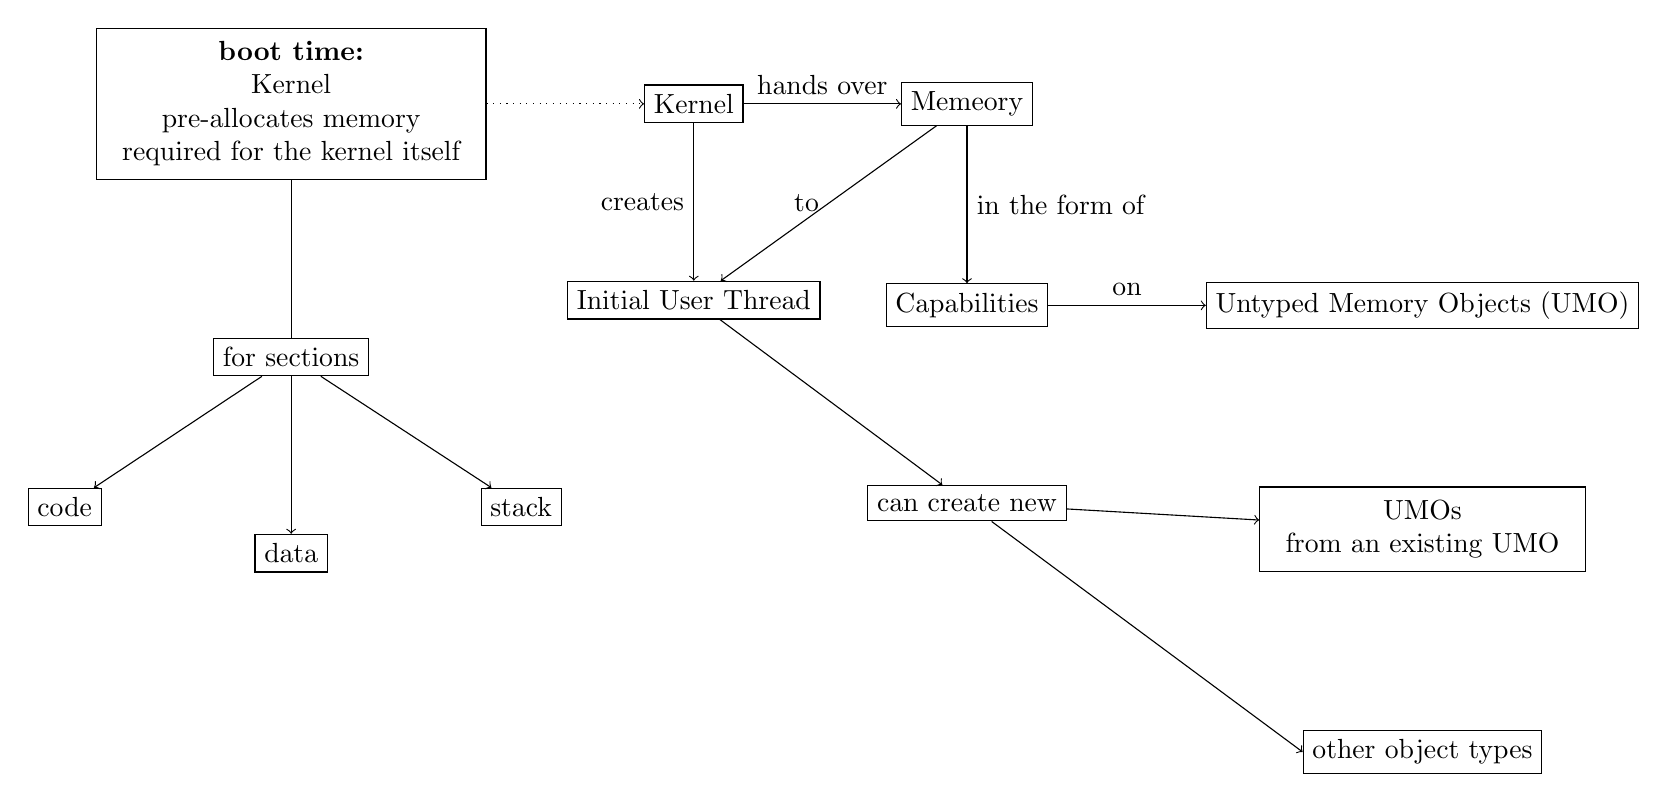
\begin{tikzpicture}[node distance=2cm]
\node[draw, rectangle](start){\begin{tabular}{c}
\textbf{boot time:} \\
Kernel \\
pre-allocates memory \\
required for the kernel itself
\end{tabular} 
  };
\node[draw, rectangle](sect)[below=of start]{for sections};
\draw[black](start)--(sect);
\node[draw, rectangle](sect1)[below left=of sect]{code};
\node[draw, rectangle](sect2)[below=of sect]{data};
\node[draw, rectangle](sect3)[below right=of sect]{stack};
\draw[->](sect)--(sect1);
\draw[->](sect)--(sect2);
\draw[->](sect)--(sect3);
\node[draw, rectangle](kernel)[right=of start]{Kernel};
\draw[dotted,->](start)--(kernel);
\node[draw, rectangle](IUT)[below=of kernel]{Initial User Thread};
\draw[->](kernel)--(IUT)node[ midway , left ] {creates};
\node[draw, rectangle](mem)[right=of kernel]{Memeory};
\draw[->](kernel)--(mem)node[ midway , above] {hands over};
\draw[->](mem)--(IUT)node[ midway , left] {to};
\node[draw, rectangle](caps)[below=of mem]{Capabilities};
\draw[->](mem)--(caps)node[ midway , right] {in the form of};
\node[draw, rectangle](umo)[right=of caps]{Untyped Memory Objects (UMO)};
\draw[->](caps)--(umo)node[ midway , above] {on};
\node[draw, rectangle](new)[below=of caps]{can create new};
\node[draw, rectangle](umos)[below=of umo]{\begin{tabular}{c}
UMOs \\
from an existing UMO
\end{tabular}};
\node[draw, rectangle](obj)[below=of umos]{other object types};
\draw[->](IUT)--(new);
\draw[->](new)--(umos);
\draw[->](new)--(obj.west);
\end{tikzpicture}
\end{document}